\begin{figure}
\begin{fullwidth}
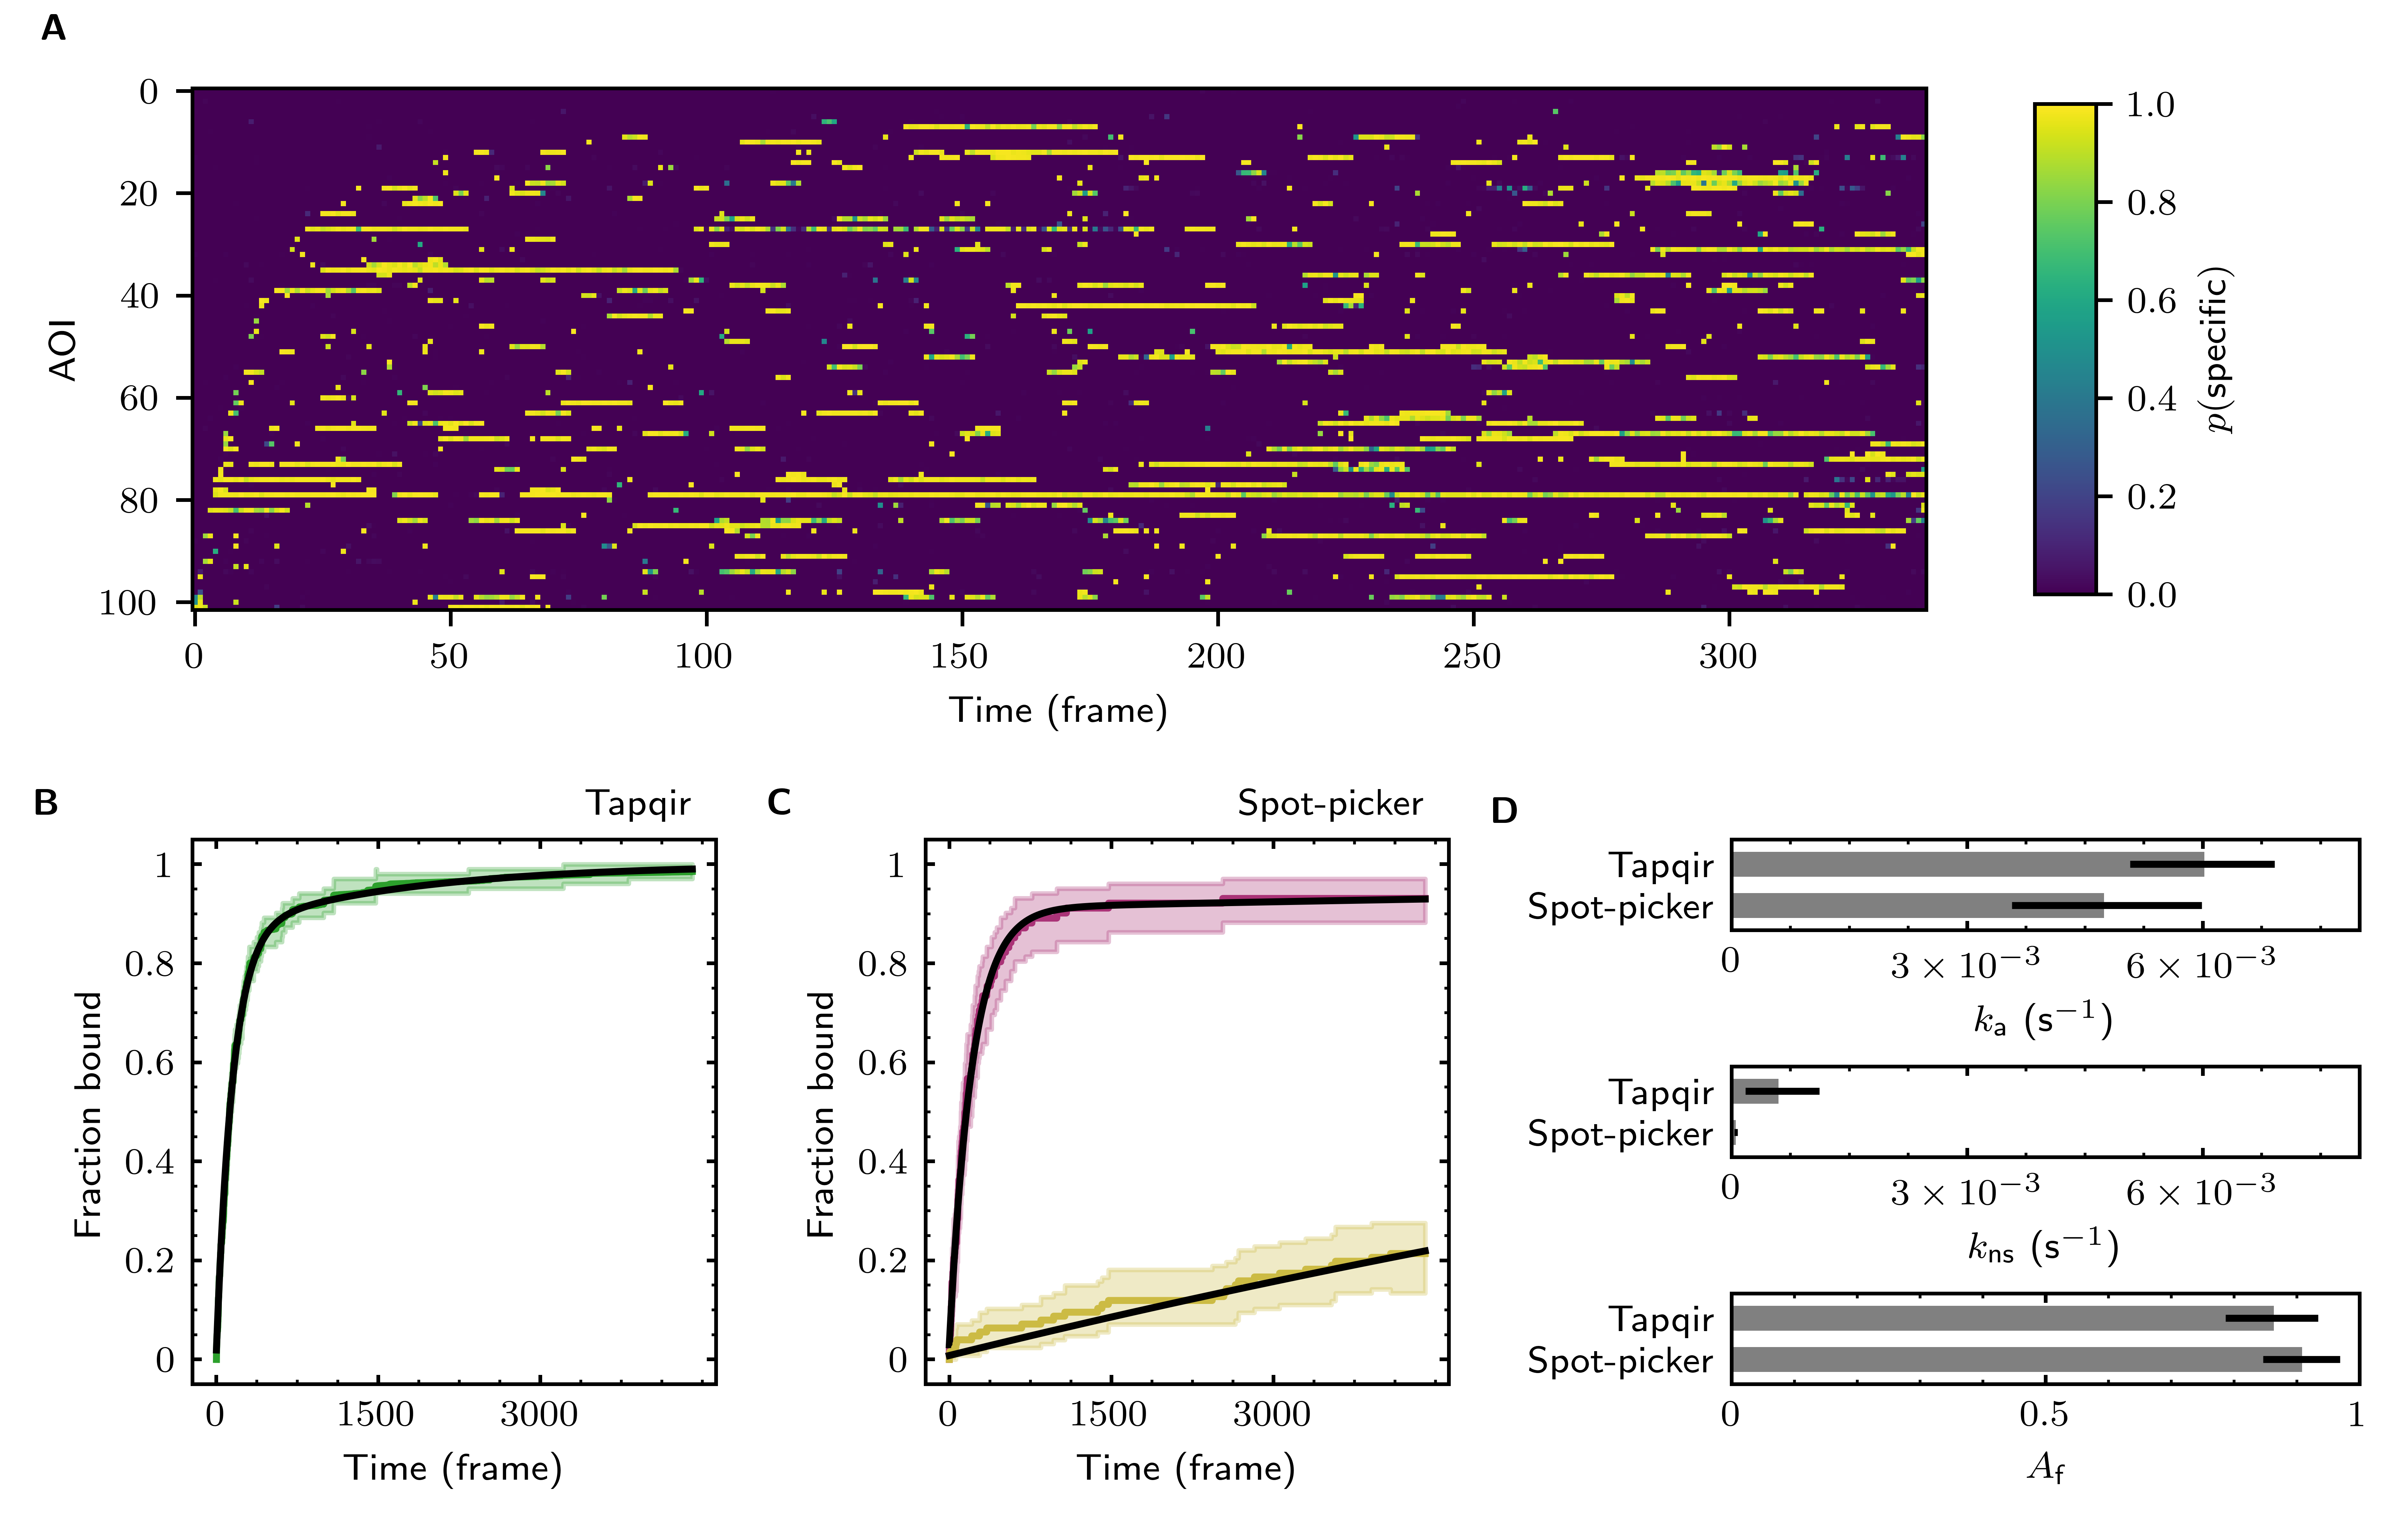
\includegraphics[width=183mm]{figures/experimental_data.png}
\caption{\textbf{Extraction of target-binder association kinetics from example experimental data.} Data are from Data set B (SNR = 3.43, $\lambda$ = 0.1290; see \TABLE{datasets}).  (\textbf{A}) Probabilistic rastergram representation of Tapqir-calculated target-specific spot  probabilities $p(\mathsf{specific})$ (color scale). AOIs were ordered by decreasing times-to-first-binding. For clarity, only every thirteenth frame is plotted. (\textbf{B}) Time-to-first-binding distribution using Tapqir. Plot shows the cumulative fraction of AOIs that exhibited one or more target-specific binding events by the indicated frame number (green) and fit curve (black). Shading indicates uncertainty. (\textbf{C}) Time-to-first-binding distribution using an empirical spot-picker method \cite{Friedman2013-sf}. The spot-picker method jointly fits first spots observed in off-target control AOIs (yellow) and in on-target AOIs (purple) with fit curves (black). (\textbf{D}) Values of kinetic parameters  $k_\mathsf{a}$, $k_\mathsf{ns}$, and $A_\mathsf{f}$ (see text) derived from fits in (\textbf{B}) and (\textbf{C}). Uncertainties reported in (\textbf{B, C, D}) represent 95\% credible intervals for Tapqir and 95\% confidence intervals for spot-picker (see Methods).
}
\label{fig:experimental_data}
\figsupp[Additional example showing extraction of target-binder association kinetics from experimental data.]{\textbf{Additional example showing extraction of target-binder association kinetics from experimental data.} Data are from Data set A (SNR = 1.63, $\lambda$ = 0.2958; see \TABLE{datasets}).  Results are plotted as in \FIG{experimental_data}, except that for clarity only every $2^\mathrm{nd}$ frame and every $3^\mathrm{rd}$ AOI is shown in (\textbf{A}).}{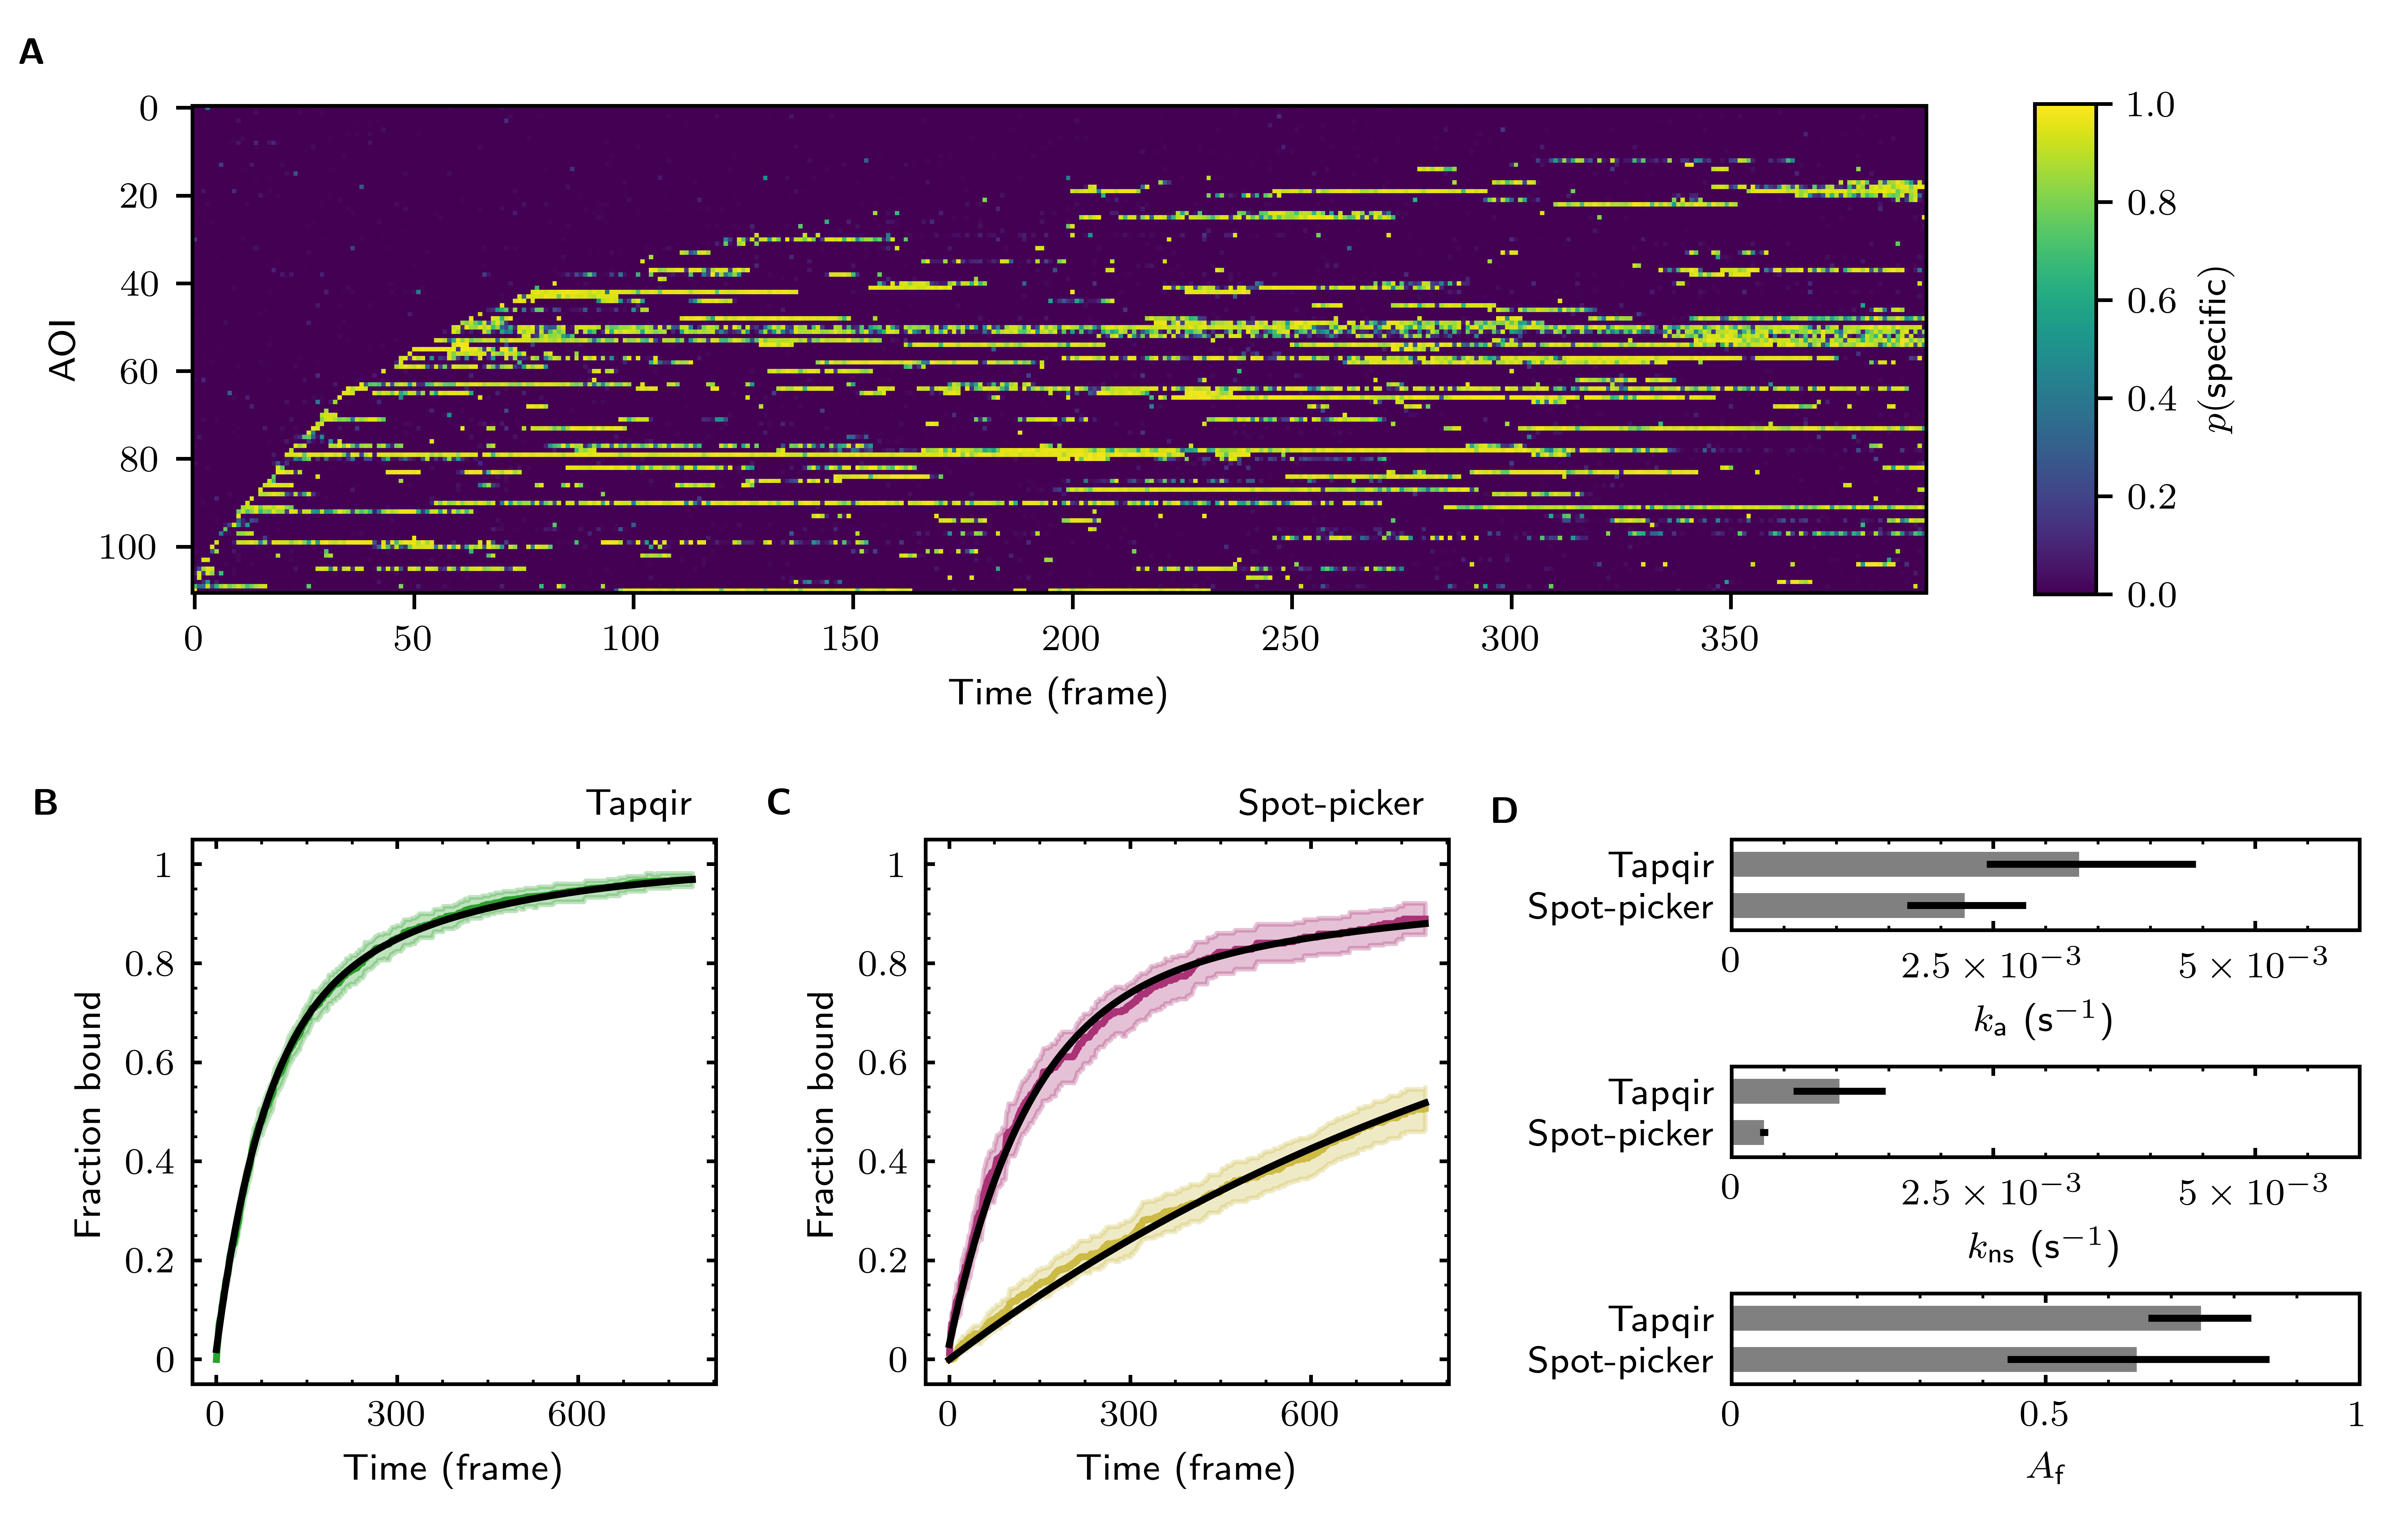
\includegraphics[width=183mm]{figures/experimental_data_DatasetA.png}}\label{figsupp:DatasetA}

\figsupp[Additional example showing extraction of target-binder association kinetics from experimental data.]{\textbf{Additional example showing extraction of target-binder association kinetics from experimental data.} Data are from Data set C (SNR = 4.18, $\lambda$ = 0.0716; see \TABLE{datasets}).  Results are plotted as in \FIG{experimental_data}, except that for clarity only every $10^\mathrm{th}$ AOI is shown in (\textbf{A}).}{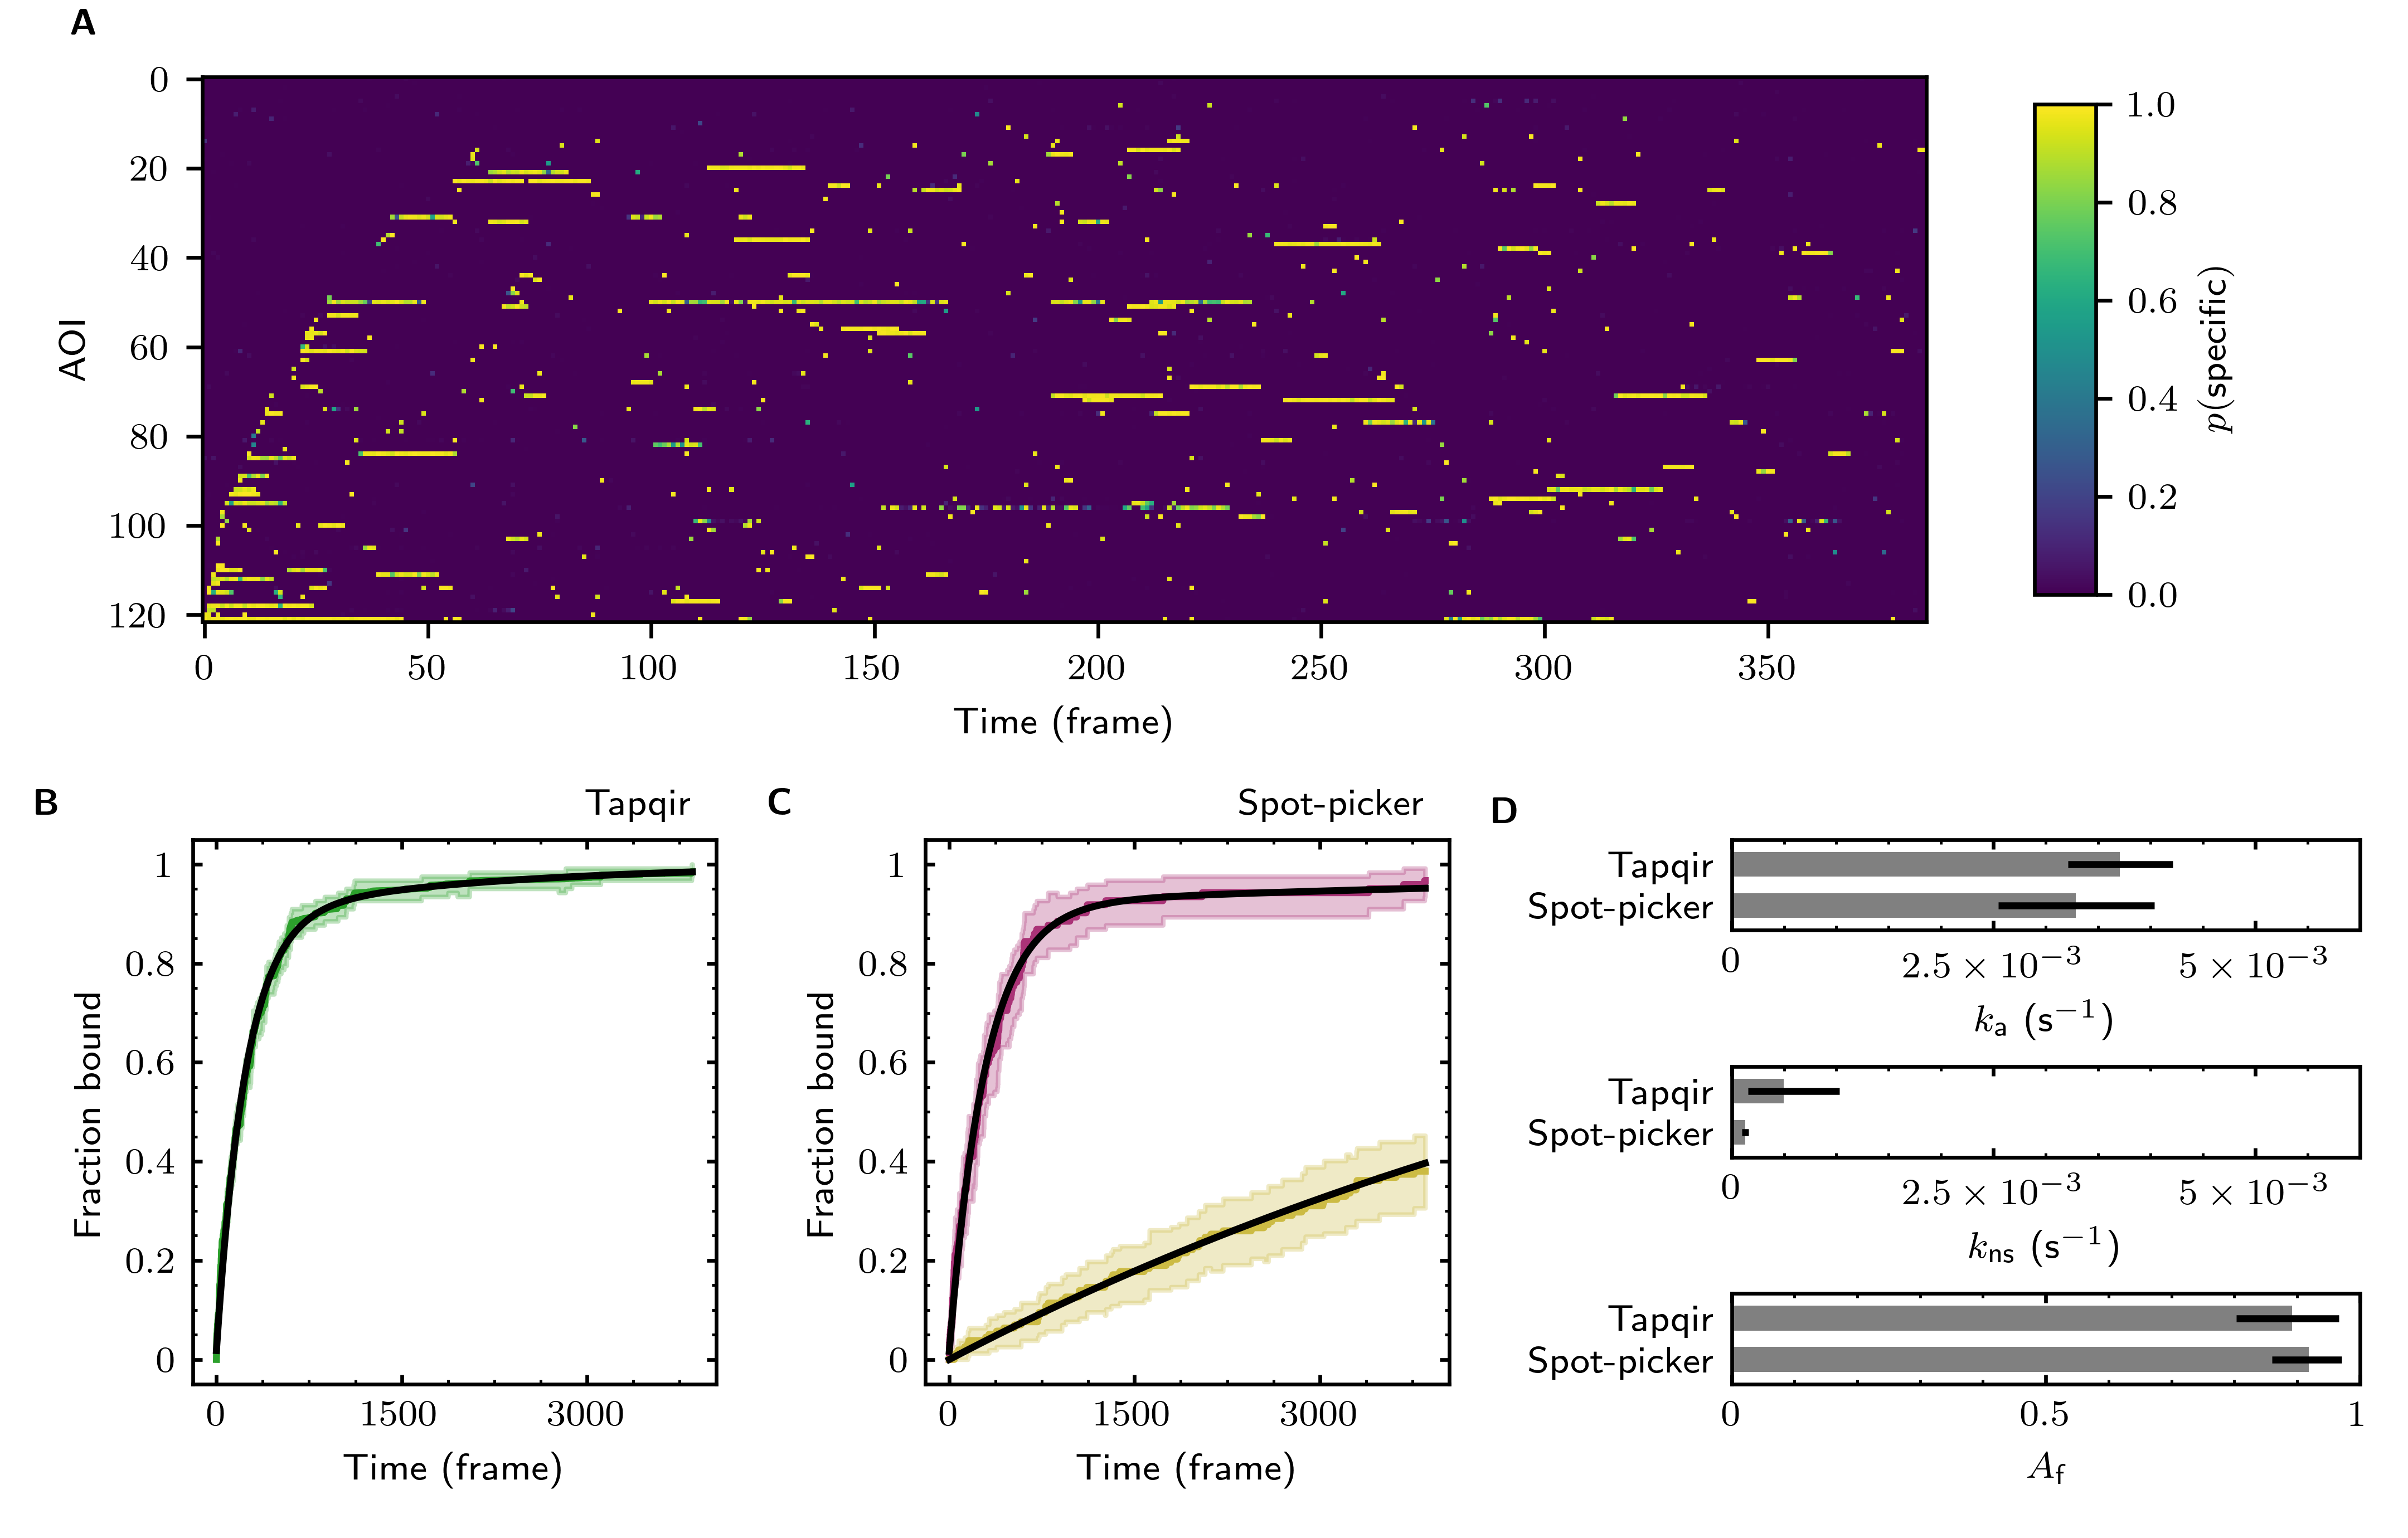
\includegraphics[width=183mm]{figures/experimental_data_DatasetC.png}}\label{figsupp:DatasetC}

\figsupp[Additional example showing extraction of target-binder association kinetics from experimental data.]{\textbf{Additional example showing extraction of target-binder association kinetics from experimental data.} Data are from Data set D (SNR = 3.14, $\lambda$ = 0.0476; see \TABLE{datasets}).  Results are plotted as in \FIG{experimental_data}, except that for clarity only every $13^\mathrm{th}$ AOI is shown in (\textbf{A}).}{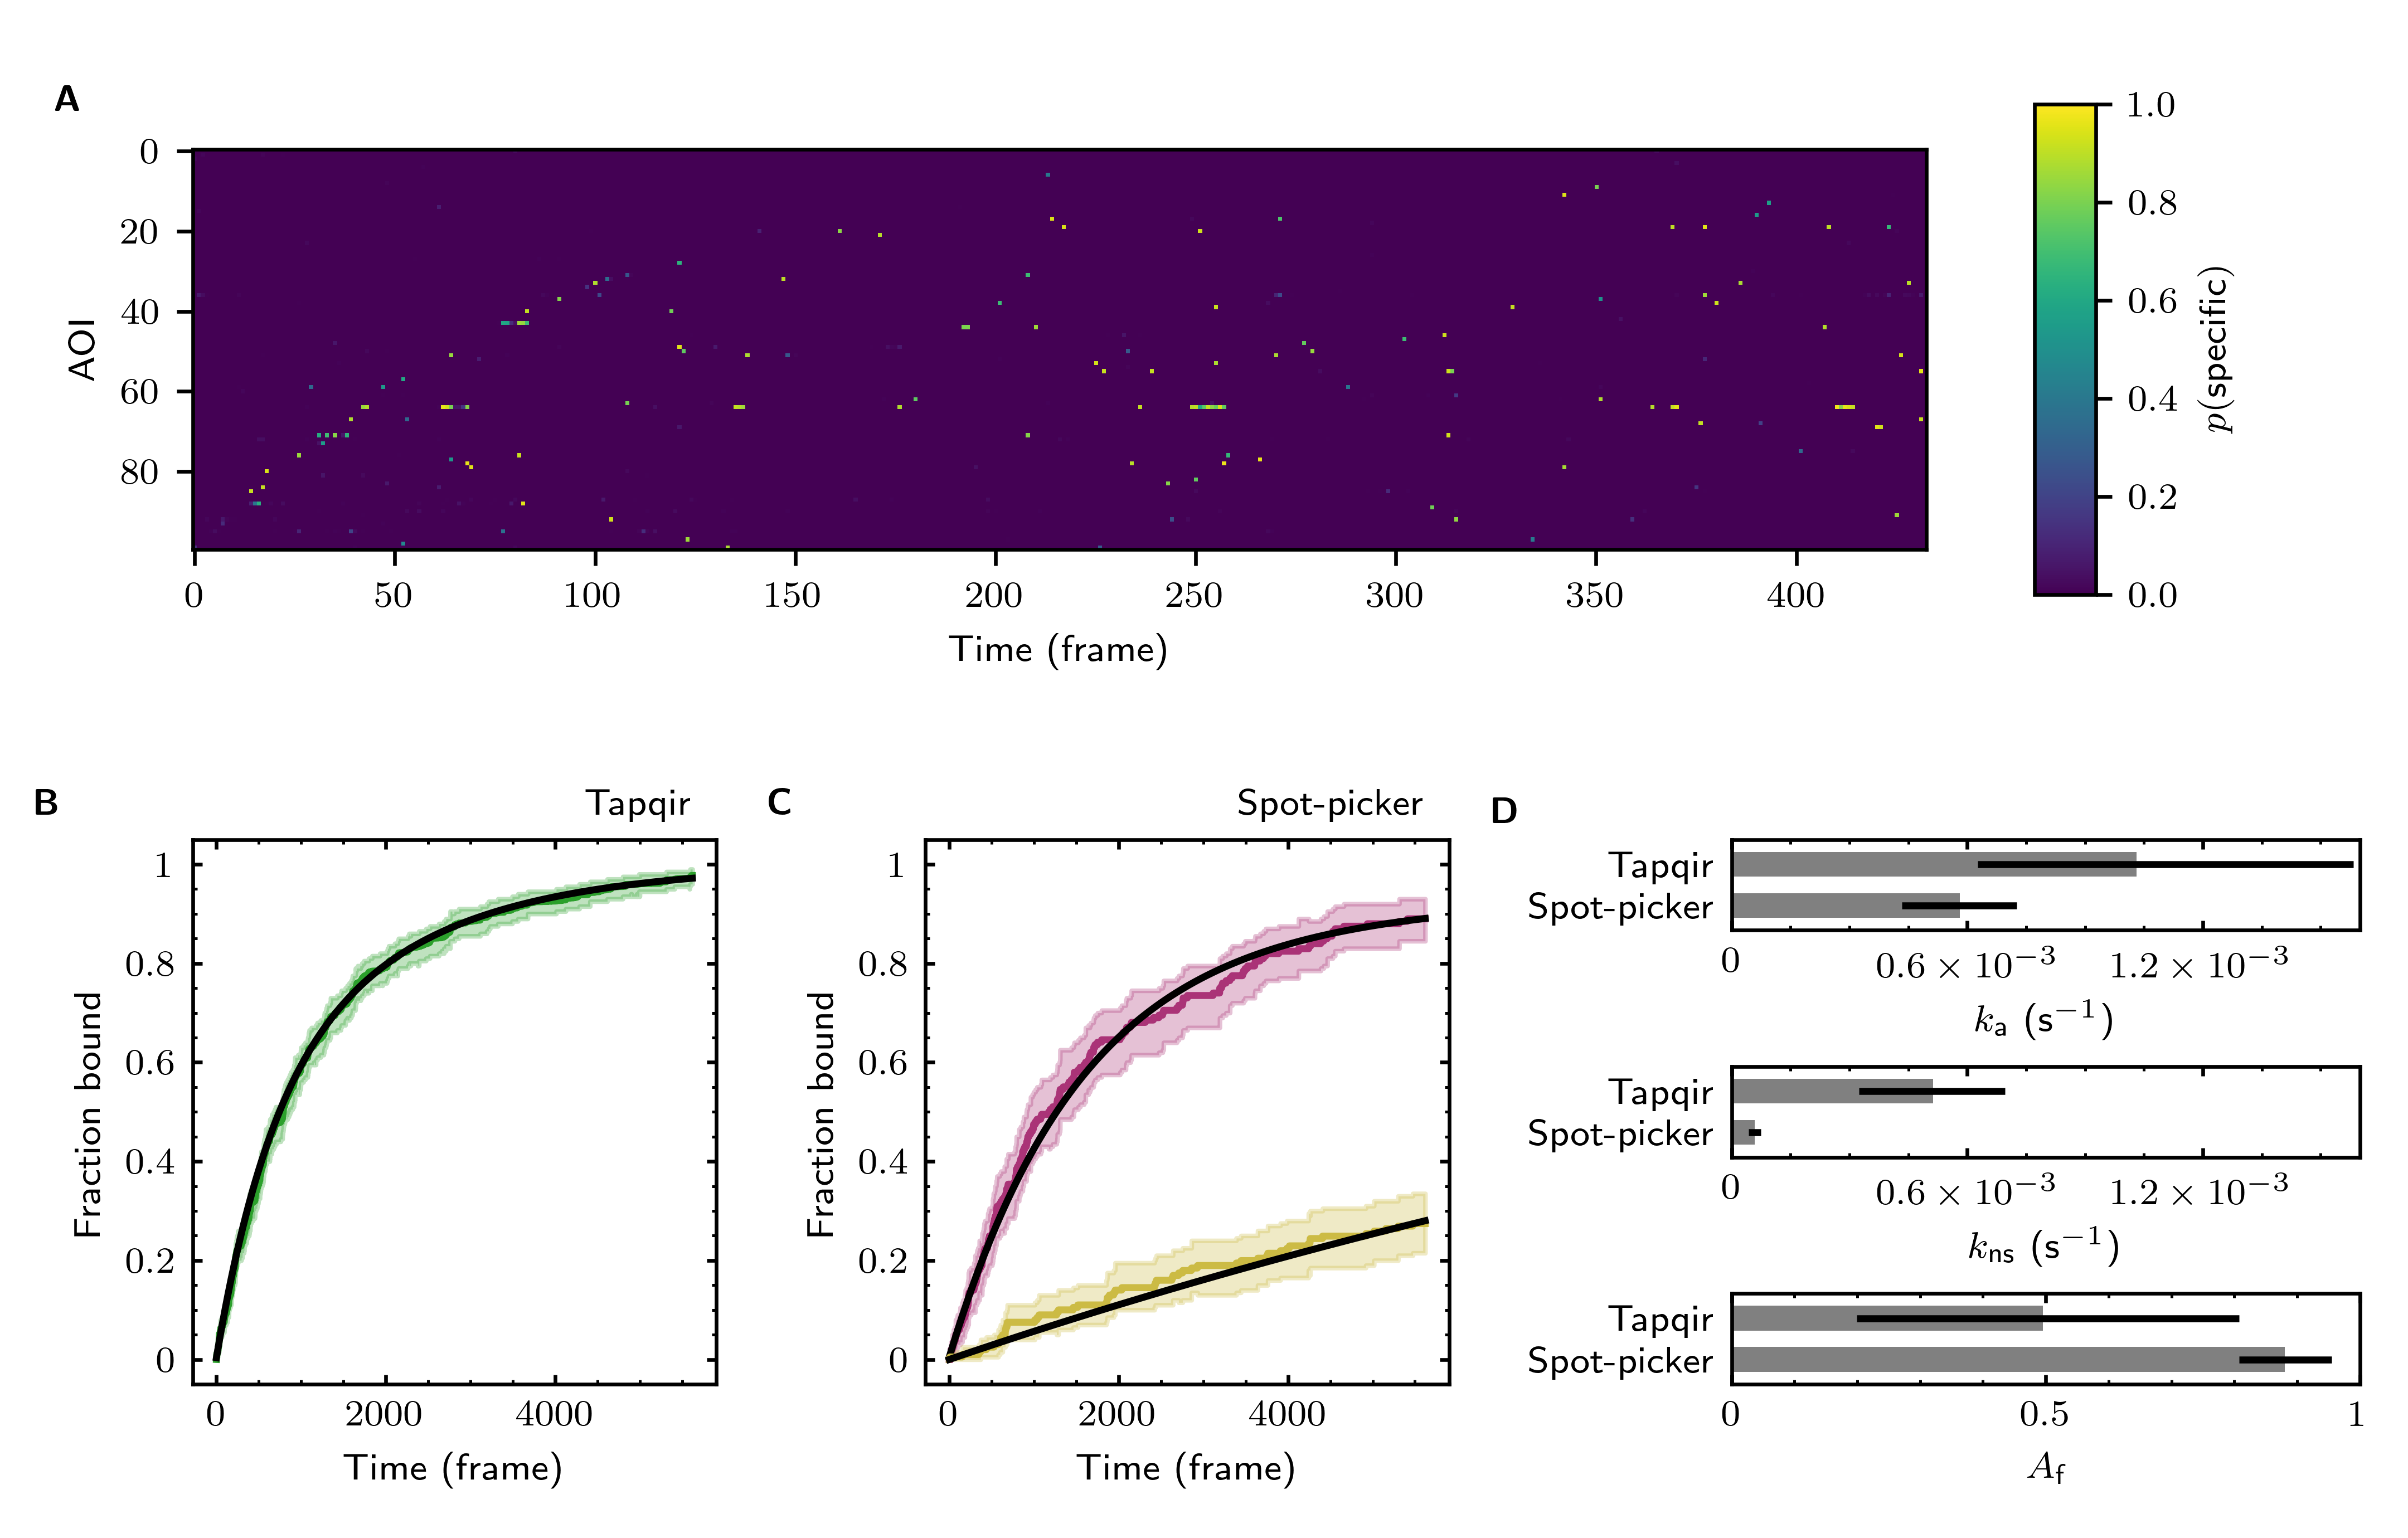
\includegraphics[width=183mm]{figures/experimental_data_DatasetD.png}}\label{figsupp:DatasetD}
\end{fullwidth}
\end{figure}